\documentclass[10pt]{book}
\usepackage[utf8]{inputenc}
\usepackage[italian]{babel}
\usepackage{multicol}
\usepackage[bookmarks]{hyperref}
\usepackage[a4paper, total={18cm, 25cm}]{geometry}
\usepackage{listings}
\usepackage{graphicx}
\usepackage{makecell}
\graphicspath{ {./img/} }
\usepackage{color}

\begin{document}
\renewcommand*\contentsname{Indice}
\title{Gestione di Reti}
\author{Federico Matteoni}
\date{A.A. 2019/20}
\maketitle
\tableofcontents
\pagebreak
\section*{Introduzione}
\paragraph{Perché bisogna studiare la gestione?} La situazione corrente comprende: un aumento delle risorse strategiche informative, le reti di computer che da strumento di supporto sono diventate elemento chiave delle organizzazioni, l'aumento esponenziale dei dispositivi interconnessi e aumento anche della complessità e delle funzionalità.\\
C'è quindi richiesta di servizi di rete permanenti e di qualità ottimale, oltre alla necessità di ridurre i costi per le infrastrutture di rete di un'azienda.
\paragraph{Necessità} Gestione di reti eterogenee con l'aiuto dei computer.
\section*{Terminologia e concetti fondamentali}
\paragraph{Managed Objects} Il controllo, la coordinazione e il monitoraggio delle risorse avviene tramite la manipolazione dei cosiddetti \textbf{managed objects}: un MO è una visione astratta di una risorsa che presenta le proprietà dal punto di vista della gestione. Sono \textbf{rappresentazioni astratte di risorse reali}.\\
I confini di un MO specificano quali dettagli sono accessibili ai sistemi di monitoraggio e quali sono schermati (\textbf{black box})

\begin{center}
Management-System $\leftrightarrow$ Managed Object $\leftrightarrow$ Real Object
\end{center}
\begin{list}{}{\textbf{Caratteristiche}}
	\item \textbf{Attributi}: descrivono lo stato/condizione dell'MO, possono cambiare quando cambia lo stato dell'oggetto reale e possono essere manipolati attraverso operazioni di management
	\item \textbf{Operazioni}: consentono l'accesso all'MO. Operazioni tipiche sono get, set, create e delete, ma il numero e tipo delle operazioni influenzano perfomance e complessità dell'oggetto
	\item \textbf{Comportamento}: determina la semantica e l'interazione con la risorsa reale. Normalmente definito in linguaggio naturale
	\item \textbf{Notifiche}: quantità e tipologia dei messaggi, che possono essere generati da situazioni pre-definite da un MO quando avviene una specifica situazione
\end{list}
\paragraph{Management Information Base} L'unione di tutti i MO contenuti in un sistema forma la MIB del sistema. La \textbf{Management Information Base} è la collezione di tutti i management object all'interno del sistema, con i loro attributi.\\
Una MIB deve essere conosciuta sia da chi la implementa che da chi la gestisce.
\subparagraph{Modularità} Gli MO di un sistema sono solitamente definiti in più MIB. Nelle MIB sono introdotti i moduli per consentire un design modulare: moduli diversi possono essere definiti da team diversi, le funzionalità di gestione possono essere estese e modificate\ldots
\paragraph{Paradigma Gestore/Agente}
\begin{list}{}{Agent}
	\item Implementa i MIB delle MO accedendo alle risorse reali
	\item Riceve le richieste da un gestore, le processa e trasmette le risposte appropriate
	\item Smista le notifica riguardanti cambiamenti di stato importanti nel MIB
	\item Protegge gli MO da accessi non autorizzati usando regole di controllo degli accessi e autenticazione della comunicazione
\end{list}
\begin{list}{}{Manager}
	\item Esercita il controllo delle funzioni
	\item Avvia operazioni di gestione tramite opportune operazioni del protocollo per la manipolazione degli MO
	\item Riceve messaggi dagli agenti e li inoltra alle applicazioni interessate per la gestione
\end{list}
\paragraph{Management Protocol} Un protocollo di gestione implementa l'accesso a MO distanti attraverso la codifica di dati di gestione (management data)
\section{lezione 2}
Livello 2 consente di identificare un device sulla rete. In tutte le reti c'è la necessità di identificare la porta di rete. Ogni dispositivo ha almeno un'interfaccia di rete: loopback, che consente di far comunicare processi di rete sulla stessa macchina. \texttt{127.0.0.1} consente di parlare su stessa macchina senza trasmettere sul filo, fondamentalmente un cortocircuito.\\
\texttt{ifconfig} consente di vedere le interfacce di rete disponibili su unix.\\
Se si vuole gestire una rete è fondamentale la standardizzazione.\\\\
Output \texttt{ifconfig}. Parte degli indirizzi, no indirizzo hw su loopback perché il traffico non esce mai (loopback sulla pila OSI è nel livello 3 Network, il MAC address è sul livello 2 Data Link, che non viene toccato da loopback). Indirizzo MAC 6 byte divisi in blocchi dai due punti. I primi 3 identificano il costruttore della scheda di rete. I successivi tre identificano la scheda di rete per il costruttore, che lo setta univocamente. Ciò garantisce univocità. Per primo blocco di tre ho 16M di dispositivi possibili. I MAC address quindi \textbf{non sono univoci}, lo sono \textit{probabilmente}. L'univocità è fondamentale sulla stessa rete. Quindi indirizzo hw identifica univocamente device sulla rete locale. divisi in due blocchi, il primo identifica costruttore della scheda di rete.\\\\
Qualsiasi dispositivo ha indirizzo hw diverso per ciascuna porta.
\section{Ethernet}
Ethernet è un cavo seriale, trasmissione e ricezione. Mezzo seriale. Un filo.\\
Quando si mandano dati non posso tutti insieme ma man mano. Non c'è collisione perché ricezione e trasmissione sono su due fili separati.\\
Pacchetti inviati nel tempo sul filo. Vengono distinti tra loro dal \texttt{preamble}. Pacchetti inviati in una direzione: preambolo, destinazione, sorgente, tipo dei dati, dati effettivi, padding (per rendere pacchetto di 64 se pacchetto è troppo corto), CRC.\\
Quindi per spedire pacchetto necessito di indirizzi (chi voglio e chi sono) e cosa mandare. chi sono lo so, è scritto nella scheda. Voglio conoscere indirizzo di chi voglio.\\
Alla connessione del cavo, se DHCP manda fuori pacchetto per richiesta quindi switch lo impara, se IP statico manda pacchetto ARP quindi switch lo impara.\\
MAC address randomizzato per privacy, spesso e volentieri sui dispositivi mobili.\\
Possibile più di un utente sulla stessa rete con soliti indirizzi, apparati avanzati se ne accorgono.
\section{lezione 3}
un pacchetto è interamente creato dal computer, quindi "non ci si può fidare"\\
Bisogna andare a livello fisico e autenticare, un po' come chiedere la carta d'identità. Metter in atto meccanismi che impediscano di inibire riconoscimento della sorgente.\\
802.1x permette di entrare in rete. Se configurato, il device prima di entrare in rete espone delle credenziali (utente, password, protocollo autenticazione\ldots)\\
Da quel momento in poi \textbf{allegato} al pacchetto c'è il mio nome, ma le informazioni di autenticazione non fanno parte del pacchetto: pacchetti creati quando non c'era preoccupazione e interesse in fattori di sicurezza delle trasmissioni.\\
L'informazione non è parte del pacchetto ma lo riconosce in qualche altro modo il device e \textbf{rimane nel device} (Access Point). Ciò non serve per autenticazione fisica sul cavo: so che sei tu su questo cavo. Ma è necessaria per autenticazione su mezzi condivisi (wifi).\\
Su router MAC cambia ad ogni hop (ethernet comunicazione punto-punto), IP cambia solo se c'è NAT. Le parti da lv 3 in su non cambiano (a meno di frammentazioni\ldots)\\
Robustezza delle reti si fa tramite la ridondanza. Tipico mettere più strade per spedire il traffico: load balancing.\\
Vale sia per corrente elettrica che per traffico di rete.\\\\
\subsection{Aree funzionali}
FCAPS per gestire \textbf{qualsiasi sistema}, da giochi a sistemi di rete. Non sono mutualmente indipendenti.
\begin{list}{}{}
	\item \textbf{Fault Management}: error detection, isolation and repair\\
	Se qualcuno rileva malfunzionamento (riempito disco, ram, sovraccarico CPU\ldots) lo deve notificare
	\item \textbf{Configuration Management}: devo sapere com'è configurato il sistema. Leggere la configurazione è importante, così che le app si possano basare sulle API comuni e funzionare correttamente. Fondamentale capire la configurazione perché permette di definire l'amministrazione, servizi\ldots, possibile riconoscere anche le adiacenze e "questo filo qui va su questa porta qua". che impatto ho se stacco questo cavo, o si rovina? Informazioni sufficenti per amministrare la rete
	\item \textbf{Account Management}: rilevare il consumo di risorse
	\item \textbf{Performance Management}: efficenze e statistiche, performance di sistema sia lato utente sia lato fornitore. Per l'utente è riuscire ad usare la rete, per l'operatore è il giusto compromesso tra investimento sul mezzo e contentezza utente.
	\item \textbf{Security Management}: assicurarsi che ciò che uno fa è effettivamente possibile farlo, autoproteggendosi perché con le reti odierne posso intasare rete (volente o no) e quindi intasare internet, provocando danni
\end{list}
\subsection{Interagire con management object}
Primitive: get, set, create, delete\\
Quando faccio richiesta ad un protocollo mi aspetto una risposta: richiesta -- risposta\\
Contenuto richieste varia durante il transito aggiungendo determinate informazioni. Es: SMS durante il transito aggiunge numero mittente per poter comunicare a destinatario chi inviava.
\subsection{Servizi}
\paragraph{Confermati} Faccio richiesta $\rightarrow$ mi aspetto risposta.\\Es: Telegram/Whatsapp
\paragraph{Non confermati} Faccio richiesta e fine.\\Es: SMS
\begin{center}
	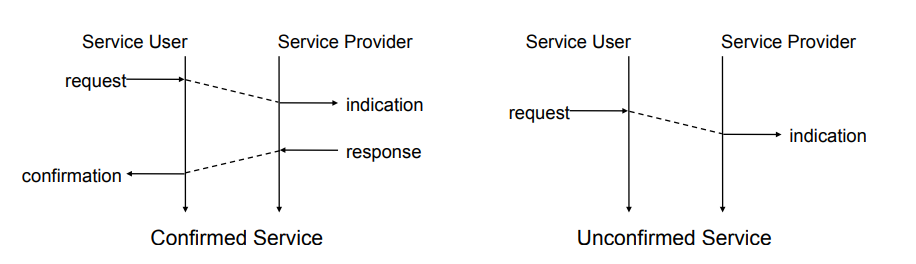
\includegraphics[scale=0.7]{timediag.png}
\end{center}
\subsection{Standardizzazione}
La grande differenza tra ISO/OSI e Internet è il processo di standardizzazione.
\pagebreak
\paragraph{ISO} Nella standardizzazione ISO tutte le varie aziende si accordano su come fare la rete: si creano gruppi di lavoro che si riuniscono (es. ICANN) e producono un documento di lavoro, poi vari comitati lo discutono (fino a qui \textbf{ad alto livello}).\\
Se si mettono d'accordo, pubblicano un \textbf{Draft International Standard} (\textbf{senza implementazione}). Dopodiché, se non viene accettato, creano technical report oppure un \textbf{full standard}.\\
La parte importante è l'assenza di implementazione fino ad avere la creazione dello standard.

\begin{center}
	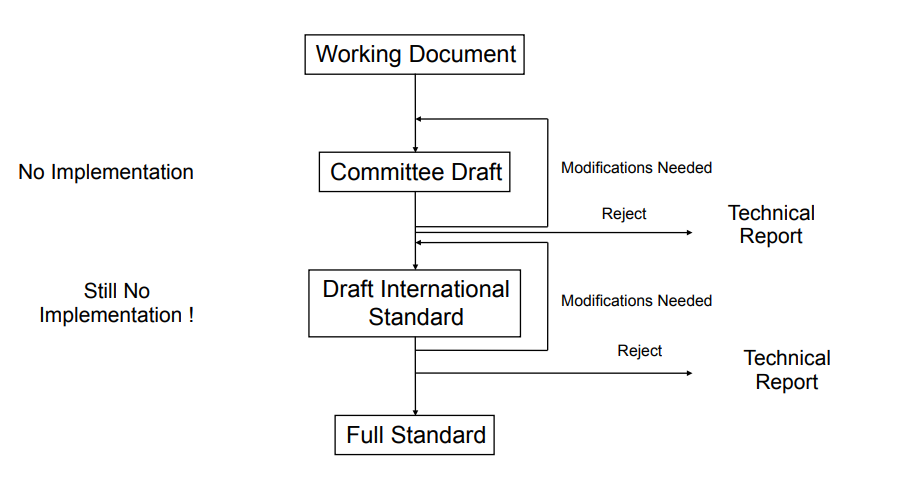
\includegraphics[scale=0.7]{stdiso.png}
\end{center}
\paragraph{Internet} Nella standardizzazione internet è tutto seguito dal comitato IETF, che pubblica aree d'interesse in cui ritiene ci sia possibilità di sviluppo. La sottomissione di un'idea ad un'area d'interesse è libera, oppure si può mandare una mail per idee completamente nuove. Dal working document a draft passa poco e i draft dopo pochi mesi scadono. Dopo massimo due anni o si rifiuta o si fa il draft standard (draft RFC) che o lo si rifiuta o diventa standard in max 4 anni. Necessita di più implementazioni interoperabili.
\begin{center}
	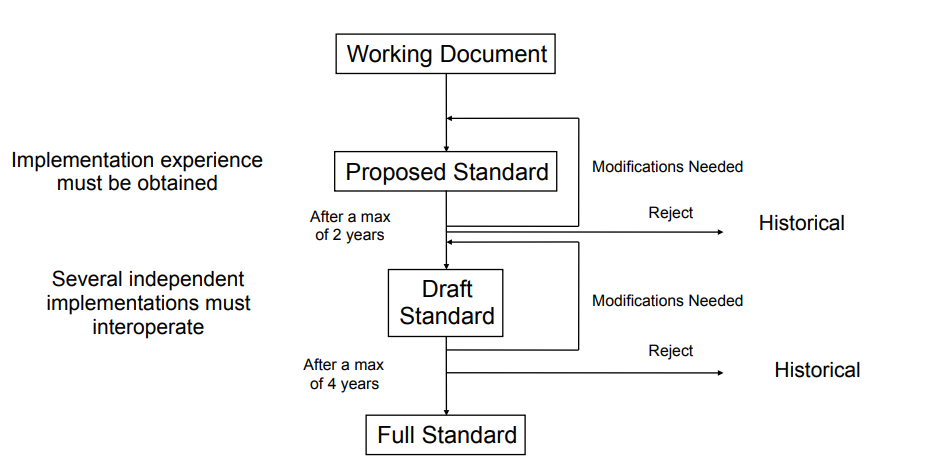
\includegraphics[scale=0.7]{stdietf.png}
\end{center}
\section{Abstract syntax notation one}
\paragraph{ASN1} Sintassi per la definizione di strutture dati e formato di messaggi. Ha l'obiettivo di consentire a macchine dalle differenti architetture hardware di scambiare dati, essere language neutral e consentire la negoziazione della codifica di trasmissione.\\
Come spostare le informazioni? Vari costruttori all'inizio lo facevano "in casa" senza interoperabilità. Col tempo si è reso necessario costruire qualcosa per scambiare le informazioni in maniera interoperabile.
\paragraph{Endian} Come si ordinano i dati in spedizione, per sapere qual è il più significativo.\\
Bit più significativo a sx è big-endian, ormai poco usato. Altrimenti è little-endian.
\end{document}